\documentclass{amsart}
\usepackage{mathtools}
\usepackage{graphicx} % Required for inserting images
\usepackage{amsmath}
\usepackage{amssymb}

%%%%%%%%%%%%%%%%%%%%
\usepackage{tikz}
\usepackage{tikz-cd}

\usepackage{tikz-3dplot}


\usepackage{pgfplots}

\pgfplotsset{%
    compat=1.8,
    compat/show suggested version=false,
}

 

\usepackage{asypictureB}


\usetikzlibrary{calc,fadings,decorations.pathreplacing}

\usepackage[many]{tcolorbox}


%%%%%%%%%%%%%%%%%%%%%%%%%%%%%%%%%%%%%%%%%%%%%


\newtheorem{theorem}{Theorem}[section]
\newtheorem{proposition}[theorem]{Proposition}
\newtheorem{corollary}[theorem]{Corollary}
\newtheorem{lemma}[theorem]{Lemma}
\newtheorem{definition}[theorem]{Definition}
\theoremstyle{remark}
\newtheorem{example}[theorem]{Example}
\newtheorem{remark}[theorem]{Remark}
\renewcommand{\refname}{References}
\renewcommand{\abstractname}{Abstract}
\numberwithin{equation}{section}

\newcommand{\tc}{\textcolor{blue}}
\newcommand{\tcg}{\textcolor{green}}
\newcommand{\RR}{\mathbb{R}}
\newcommand{\CC}{\mathbb{C}}
\newcommand{\NN}{\mathbb{N}}
\newcommand{\PP}{\mathbb{P}}

\def\mclimits_#1{\limits_{\mathclap{#1}}}








\begin{document}
\title{A remark on the Gaussian Radon transform, Pad\'e approximants, and shape reconstruction}


\date{\today}

\author[M.~Derevyagin]{Maxim~Derevyagin}
\address{
MD,
Department of Mathematics\\
University of Connecticut\\
341 Mansfield Road, U-1009\\
Storrs, CT 06269–1009, USA}
\email{maksym.derevyagin@uconn.edu}

\author[A.~Sengupta]{Ambar~Sengupta}
\address{
AS,
Department of Mathematics\\
University of Connecticut\\
341 Mansfield Road, U–1009\\
Storrs, CT 0626–91009, USA}
\email{ambar.sengupta@uconn.edu}

\author[J.~Toman–Yih]{Jasper~Toman–Yih}
\address{
JT,
Department of Mathematics\\
University of Connecticut\\
341 Mansfield Road, U–1009\\
Storrs, CT 06269–1009, USA}
\email{jasper.toman–yih@uconn.edu}

\subjclass{Primary ????; Secondary ????.}
\keywords{????; ????; ????.}

\begin{abstract}
\tc{To be done later}
\end{abstract}

\maketitle

\section{Introduction}

\tc{To be done later.}
\newpage
\section{Notation}

First recall the conventional multiindex notation. Let $\NN_0$ denote the nonnegative integers. A multiindex $\alpha = (\alpha_1, \alpha_2, \ldots, \alpha_n) \in \NN_0^n$ is an $n$-tuple of nonnegative integers. The degree of a multiindex is $|\alpha| = \alpha_1 + \alpha_2 + \cdots + \alpha_n$. Multivariate exponentiation is defined as follows. For $x = (x_1, x_2, \ldots, x_n) \in \RR^n$,
\[
    x^\alpha = x_1^{\alpha_1}x_2^{\alpha_2} \cdots x_n^{\alpha_n}.
\]
The multinomial formula gives a convenient expansion for multinomial powers. Let $k \in \NN_0$ and $b = b_1 + b_2 + \cdots + b_n$. Then
\[
    b^k = \sum_{|\alpha| = k} \binom{k}{\alpha} b^\alpha
\] 
where the multinomial coefficients are defined
\[
    \binom{k}{\alpha} = \frac{k!}{\alpha_1! \alpha_2! \cdots \alpha_n!}.
\]
Note that the multinomial expansion sums over all multiindeces $\alpha \in \NN_0^n$ of degree $k$.

We denote the standard euclidean inner product
\[
    \langle x,y \rangle = x_1y_1 + x_2y_2 + \cdots x_ny_n
\]
where $y = (y_1, y_2, \ldots, y_n) \in \RR^n$. When discussing hyperplanes in $\RR^n$ we index them by a unit normal vector, $\omega \in \RR^n$, and distance from origin $-\infty < p < \infty$, and we write for example $\langle x, \omega \rangle = p$. Note that $\langle x, -\omega \rangle = p$ is the same hyperplane. It is perhaps more correct, in later defining the Radon and Gaussian Radon transforms, to identify these indexes and define the transforms over a projective space. We omit this discussion as it is not relevant within the scope of this work.
\begin{figure}
    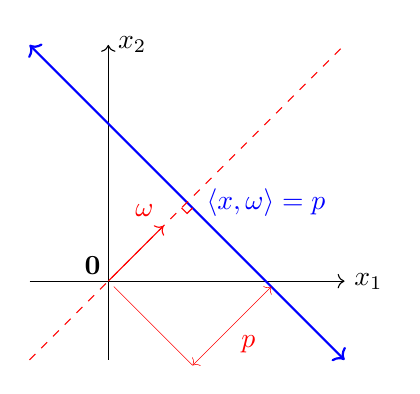
\begin{tikzpicture}[plane/.style={<->,thick,blue},
        vector/.style={->,red},
        axis/.style={->,black}]
    %draw axes
    \draw[axis] (-1,0) -- (3,0) node[anchor=west]{$x_1$};
    \node at (-.2,.2) {$\mathbf{0}$};
    \draw[axis] (0,-1) -- (0,3) node[anchor=west]{$x_2$};
    %draw plane
    \draw[plane] (-1, 3) -- (3, -1) node[midway, right]{~$\langle x, \omega\rangle = p$};
    %draw projection angle and orthogonal vector
    \draw[red,dashed] (-1,-1) -- (3,3);
    \def\ra{.07};
    \draw[red] (1-\ra, 1-\ra) -- (1,1-2*\ra) -- (1+\ra,1-\ra);
    \draw[vector] (0,0) -- (0.7,0.7) node[above left]{$\omega$};
    %draw extension line
    \draw[very thin, red] (\ra, -\ra) -- (1+\ra, -1-\ra);
    \draw[<->,very thin, red] (1+\ra, -1-\ra) -- (2+\ra, -\ra) node[midway,below right]{$p$};
    \end{tikzpicture}
\end{figure}

Unless otherwise indicated all measures are Euclidean measures, that is the Borel measure assocciated with the standard Euclidean metric on a given space. In particular the Euclidean measure on a hyperplane of $\RR^n$ is equivalent to the Euclidean measure on $\RR^{n-1}$. We chose for convenience to denote measures by their associated variable such as $dx$, $dp$, $dz$, and others. It should be stated that this notation, while uniform, is context dependent; it is a loving abuse of notation. For example in the integrals
\[
    \int_{\RR^n}~dx \qquad \text{and} \qquad \int_{\langle x, \omega\rangle = p} ~dx,
\]
the measure $dx$ is to be understood as the $n$-dimensional and $(n-1)$-dimensional Euclidean measure respectively.

\newpage
\section{Classical and Multivariate Moments}

Let $f(x)$ be a measurable function on $\RR$. For $k \in \NN_0$, define the $k$th moment of $f$ as
\[
    c_k = \int_{-\infty}^\infty f(x)x^k ~dx.
\]
The sequence $(c_k)_{k \in \NN_0}$ is called a moment sequence or a moment problem, and the function $f$ is called a solution to the moment problem. Loosly speaking a moment problem poses the question: Under given constraints (e.g. domain, continuity, etc...), to what extent can one determine the solution $f$ from its moments?

The classical study of moment problems is divided into three cases depending on the domain: 
\begin{enumerate}
\item Markov (or Haussdorf) moment problems for bounded domains (i.e. the unit interval), 
\item Stieltjes moment problems for one-sided unbounded domains (i.e. the positive real line), and 
\item Hamburger moment problems for bi-infinite domains (i.e. the real line).
\end{enumerate}

There are two natural questions one can ask about a moment problem:
\begin{enumerate}
\item Solvability: Does a solution $f$ exist possessing the given moments?
\item Determinacy: Is a solution unique? If not, what can be said about the set of solutions?
\end{enumerate}
In the classical cases (Markov, Stieltjes, Hamburger) these questions have been resolved. Precise conditions for solvable and determinate moment problems exist, and the nature of solution sets to indeterminate moment problems are well understood. For instance, in the class of continuous functions on the unit interval, all solvable moments problems are determinate. However many classes of generalized moment problems remain in active study.

In particular let us discuss multivariate moment problems. Let $f(x)$ be a measureable function now on $\RR^n$. For $\alpha \in \NN_0^n$, define the $\alpha$th multivariate moment of $f$ as 
\[
    c_\alpha = \int_{\RR^n} f(x)x^\alpha ~ dx.
\]
The moment sequence $(c_\alpha)_{\alpha \in \NN_0^n}$ is now multiindexed. No precise general conditions are known for the solvability or determinacy of multivariate moment problems. However some sufficient conditions have been discovered by leveraging classical moment problem theory. 

\newpage
\section{Basics of the Radon and Gaussian Radon transforms}

Let $f$ be a multivariable function on the $n$-dimensional Euclidean space $\RR^n$. We imagine taking "slices" of $f$ by restricting it to a $(n-1)$-dimensional hyperplane $\Lambda$. These hyperplanes form the domain of the Radon Transform. More precisely, the Radon Transform associates each slice with a corresponding integral
\[
    R_f(\Lambda) = \int_{\Lambda} f(x) ~dx,
\]
which can be thought of as a $(n-1)$-dimensional measurement of $f$. To be more precise we parametrize the collection of hyperplanes $\Lambda$ by unit normal vector, $\omega \in \RR^n$, and (signed) distance from the origin $-\infty < p < \infty$. Indeed any hyperplane can be described in the form $\Lambda = \{x \in \RR^n: \langle x, \omega\rangle = p\}$.

\begin{definition}
    Let $f$ be a positive measurable function on $\mathbb{R}^n$. The \textbf{Radon transform} (\textbf{RT}) of $f$ is a function which, given a unit vector $\omega \in \RR^n$ and $-\infty < p < \infty$, is defined as
    \[
        R_f(\omega, p) = \int\mclimits_{\langle x, \omega \rangle = p} f(x) ~dx,
    \]
    provided the integral converges.
\end{definition}

Our main addition to previous work will be the use of a modified RT, the Gaussian Radon transform. This transform is very similar to the RT, but the inclusion of a Gaussian weight in the integral allows for convergence on a larger class of functions $f$.

\begin{definition}
The \textbf{Gaussian Radon transform} (\textbf{GRT}) of $f$ is defined similarly to the RT. Given a unit vector $\omega \in \RR^n$ and $-\infty < p < \infty$, the GRT is
\[
    GR_f(\omega, p) = 
    \int\mclimits_{\langle x, \omega \rangle = p} f(x) e^{-\frac{\|x - p\omega\|^2} 2} ~dx.
\]
provided the integral converges. Note the weighting function $e^{-\|x - p\omega\|^2/2}$ is centered on the point of the hyperplane closest to the origin, $p\omega$.
\end{definition}

\begin{remark}
It may be helpful to understand the GRT as a simple modification of the RT with respect to a Gaussian measure on $\RR^n$. Let $g(x) := f(x)e^{-\|x\|^2/2}$. The RT of $g$ can be rewritten
\begin{align*}
    \int\mclimits_{\langle x, \omega \rangle = p} f(x) e^{-\frac{\|x\|^2} 2} ~dx
    &= \int\mclimits_{\langle x, \omega \rangle = p} f(x) e^{-\frac{\|x - p\omega\|^2} 2} ~dx~ e^{-\frac{\|p\omega\|^2} 2},
\end{align*}
where we used the Pythagorean relation $\|x\|^2 = \|x - p\omega\|^2 + \|p\omega\|^2$. Since $\omega$ is a unit vector, $\|p\omega\|^2 = p^2$. In short, we have proved the formula
\begin{equation}
    \label{eq:1}
    R_g(\omega, p) = GR_f(\omega, p)e^{-\frac{p^2} 2}, \qquad g(x) := f(x)e^{-\frac{\|x\|^2} 2}.
\end{equation}
The relation above provides decent intuition for the GRT, and is also a useful tool proving some basic properties of the transform.
\end{remark}

\[
    \int_{-\infty}^\infty R(\omega, p) ~dp = \int_{\RR^n} f(x) ~dx
\]
The so called "slice theorem" generalizes further generalizes this observation.
% In fact, the following "slice theorem" gives a formula for integrating a projection against any weighting function $F(p)$, assuming the integral converges. 
\begin{theorem}[Slice Theorem]
    If $\int_{\mathbb{R}^n} |f(x) F(\langle x, \omega \rangle)| dx < \infty$ then
    \begin{align}
        \label{eq:ST}
        \int_{-\infty}^\infty R_f(\omega, p) F(p) dp 
        % &= \int_{-\infty}^\infty \int_{\langle x, \omega \rangle = p} f(x) F(p) ~d\mu(x) ~dp 
        &= \int_{\mathbb{R}^n} f(x) F(\langle x, \omega \rangle) dx.
    \end{align}
\end{theorem}

\begin{proof}
Inserting the definition of the RT, the left side is
\[
    \int_{-\infty}^\infty \int\mclimits_{\langle x, \omega \rangle = p} f(x) ~dx~ F(p) ~dp 
    = \int_{-\infty}^\infty \int\mclimits_{\langle x, \omega \rangle = p} f(x) F(\langle x, \omega \rangle) ~dx dp.
\]
Up to a rigid transformation (under which the Euclidean measures are invariant) this is essentially an itterated integral over $\RR$ and $\RR^{n-1}$. Thus given the integrability requirement, Fubini's theorem applies and the theorem is proved.
\end{proof}

%  We can specify various conditions for convergence of this integral, say by H\"older's inequality \tc{not very helpful on RHS, $F(\langle x, \omega\rangle)$ is not $L^p(\mathbb{R}^n)$ for $p < \infty$, $n > 1$, but LHS maybe}. If $F(p)$ is bounded then $\int |f(x)| dx < \infty$ suffices for convergence. If $f$ is continuous with compact support then $F(p)$ only needs to be integrable.

If $F(p) = e^{-ip}$ and $f(x)$ is such that $\int_{-\infty}^\infty R_f(\omega, p) dp < \infty$ then (\ref{eq:ST}) becomes the well known Fourier slice theorem
\[
    \int_{-\infty}^\infty R_f(\omega, p) e^{-ip} ~dp
    = \int_{\mathbb{R}^n} f(x) e^{-i\langle x, \omega\rangle} ~dx,
\]
which is often articulated as saying that the $1$-D Fourier transform of the Radon transform is the $N$-D Fourier transform of $f$.

By way of the relation (\ref{eq:1}) we can prove an analagous slice theorem for the GRT. 
\begin{proposition}[Gaussian Slice Theorem] If $\int_{\mathbb{R}^n} |f(x) F(\langle x, \omega\rangle) e^{-\|x\|^2/2}dx < \infty$ then
\begin{equation}\label{eq:GST}
    \int_{-\infty}^\infty GR_f(\omega, p)F(p) e^{-\frac{p^2} 2} ~dp
    = \int_{\mathbb{R}^n}f(x) F(\langle x, \omega\rangle) e^{-\frac{\|x\|^2} 2} ~dx. 
\end{equation}
% \tc{Whatever conditions are sufficient for (\ref{eq:2}) are then sufficient conditions to be checked for $g(x) = f(x)e^{-\|x\|^2}$ and $G(p) = F(p)e^{p^2}$.}
\end{proposition}
\begin{proof}
From (\ref{eq:1})
\[
    \int_{-\infty}^\infty GR_f(\omega, p)F(p) e^{-\frac{p^2} 2} ~dp 
    = \int_{-\infty}^\infty R_g(\omega, p) F(p) ~dp
\]
where $g(x) = f(x)e^{-\|x\|^2/2}$. Then applying the slice theorem:
\[
    \int_{-\infty}^\infty R_g(\omega, p) F(p) ~dp 
    = \int_{\RR^n} f(x)F(\langle x, \omega \rangle) e^{-\frac{\|x\|^2} 2} ~dx,
\]
completing the proof.
\end{proof}

% \begin{remark}
%     For an equivalent 
% \end{remark}

We will make use of two related applications of the slice theorems going forward. First we show that, fixing $\omega$, the $k$th projection moment at $\omega$ can be written as a weighted sum of the degree $k$ multivariate moments of $f$. 
\begin{proposition}
    Let $c_\alpha (\omega) = \int_{-\infty}^\infty R_f(\omega, p) p^k dp$ be the projection moments of $f$ at a fixed $\omega$, and $c_\alpha$ the multivariate moments of $f$. Then
    \[
        c_k(\omega) = \sum_{|\alpha| = k}\binom{k}{\alpha} \omega^\alpha c_\alpha
    \]
    where $\binom{k}{\alpha} = \frac{k!}{\alpha_1! \alpha_2! \cdots \alpha_n!}$ are multinomial coefficients.
\end{proposition}
\begin{proof}
By the slice theorem (\ref{eq:ST}) with $F(p) = p^k$,
\[
    \int_{-\infty}^\infty R_f(\omega, p) p^k ~dp 
    = \int_{\RR^n} f(x) \langle x, \omega \rangle^k ~dx.
\]
Now $\langle x, \omega \rangle^k = (x_1 \omega_1 + \cdots + x_n \omega_n)^k$ has the multinomial expansion
\[
    \langle x, \omega \rangle^k = \sum_{|\alpha| = k}\binom{k}{\alpha} x^\alpha\omega^\alpha.
\]
Thus after a bit of rearranging we get
\begin{align*}
    \int_{\RR^n} f(x) \langle x, \omega \rangle^k ~dx
    &= \int_{\RR^n} f(x) \sum_{|\alpha| = k}\binom{k}{\alpha} x^\alpha \omega^\alpha ~dx \\
    &= \sum_{|\alpha| = k}\binom{k}{\alpha} \omega^\alpha \int_{\RR^n} f(x) x^\alpha ~dx,
\end{align*}
where the integrands are precisely the $k$th degree multivariate moments of $f$.
\end{proof}
% \begin{align*}
%     c_k(\omega) &:= \int_{-\infty}^\infty R_f(\omega, p) p^k dp \\
%     &= \int_{\RR^n} f(x) \langle x, \omega \rangle^k dx \\
%     &= \sum_{|\alpha| = k}\binom{k}{\alpha} \omega^\alpha \int_{\RR^n} f(x) x^\alpha dx
%     =: \sum_{|\alpha| = k}\binom{k}{\alpha} \omega^\alpha c_\alpha
% \end{align*}
Similarly, moments of the GRT (Gaussian projection moments) can be expressed in terms of multivariate gaussian moments.
\begin{proposition}
Let $c_k^G(\omega) = \int_{-\infty}^\infty GR_f(\omega, p) p^k e^{-p^2/2} dp$ be the Gaussian weighted moments of the GRT of $f$ at a fixed $\omega$. Let $c^G_\alpha = \int_{\RR^n} f(x) e^{-\|x\|^2/2} x^\alpha dx$ be the Gaussian weighted multivariate moments of $f$. Then
\[
    c^G_k(\omega) = \sum_{|\alpha| = k}\binom{k}{\alpha} \omega^\alpha c^G_\alpha.
\]
\end{proposition}

\begin{proof}
The proof follows as it did for the RT. This time we apply the GRT slice theorem (\ref{eq:GST}) with $F(p) = p^k$, 
\begin{align*}
    \int_{-\infty}^\infty GR_f(\omega, p) p^k e^{-\frac{p^2}2} ~dp
    &= \int_{\RR^n} f(x) \langle x, \omega \rangle^k e^{-\frac{\|x\|^2}2} ~dx
\end{align*}
Again we use the multinomial expansion and rearange:
\[
    \int_{\RR^n} f(x) \langle x, \omega \rangle^k e^{-\frac{\|x\|^2}2} ~dx
    = \sum_{|\alpha| = k} \binom{k}{\alpha} \omega^\alpha \int_{\RR^n} f(x) e^{-\frac{\|x\|^2}2}x^\alpha dx. 
\]
Thus
\[
    c^G(\omega) = \sum_{|\alpha| = k} \binom{k}{\alpha} \omega^\alpha c^G_\alpha.
\]
% \begin{align*}
%     c_k^G(\omega) &:= \int_{-\infty}^\infty GR_f(\omega, p) p^k e^{-p^2/2} dp \\
%     &= \int_{\RR^n} f(x) e^{-\|x\|^2/2}\langle x, \omega\rangle^k dx \\
%     &= \sum_{|\alpha| = k} \binom{k}{\alpha} \omega^\alpha \int_{\RR^n} f(x) e^{-\|x\|^2/2}x^\alpha dx 
%     =: \sum_{|\alpha| = k} \binom{k}{\alpha} \omega^\alpha c_\alpha^G
% \end{align*}
\end{proof}

Finally we prove two formulas regarding the Hamburger transform of a projection, defined more preceisely in the next section. For now we note that the transform is closely related to the projection moments and has the integral representation
\[
    g(z) = \int_\infty^\infty \frac{R(\omega, p)}{1 + zp} dp
\]
By applying the slice theorem, with $F(p) = (1+zp)^{-1}$ we see that the Hamburger transform of a projection can be represented by a similar multivariable integral of $f$ over $\RR^n$.
\[
    \int_{-\infty}^\infty \frac{R_f(\omega, p)}{1 + zp} dp = \int_{\RR^n} \frac{f(x)}{1 + z\langle x, \omega \rangle} dx
\]
Similarly the GRT slice theorem with $F(p) = (1 + zp)^{-1}$ is
\[
    \int_{-\infty}^\infty \frac{GR_f(\omega, p) e^{-p^2/2}}{1 + zp} dp = \int_{\RR^n} \frac{f(x)e^{-\|x\|^2/2}}{1 + z\langle x, \omega \rangle} dx.
\]

% \tc{Is this really the assumption we want? Check more carefully.}
% For our purposes it will suffice to assume that $f(x) e^{-\|x\|^2/2}$ is bounded and $\int_{-\infty}^\infty |F(p)e^{p^2/2}| dp < \infty$.

% \tc{Or is it this?}
% One case of interest: Suppose $|f(x)| \leq M$. Then $|GR_f(\omega, p)| \leq M \sqrt{2\pi}$, and the slice theorem holds if $F(p)$ is integrable.
\newpage
\section{The Markov and Hamburger Transforms}
Let $g(z) = \int (1+zu)^{-1}d\mu$, where $\mu$ is a Borel measure with infinite support. When $\mu$ has bounded (unbounded resp.) support we call $g(z)$ the Markov (Hamburger resp.) transform of the measure $\mu$. 

The function $g(z)$ is holomorphic on the open half planes $\text{Im}~z \neq 0$ and admits a formal assymptotic expansion $\sum_{n=0}^\infty c_n(-z)^n$ — which we will call the Markov (Hamburger resp.) series — in the sense that
\begin{equation}
    g(z) = c_0 - c_1z + c_2z^2 - \cdots + c_n(-z)^n + z^n h_n(z) \label{assexp}
\end{equation}
where $\lim_{z \rightarrow 0} h_n(z) = 0$ non-tangentially for all $n = 0, 1, \ldots$.


We first note that 
\[
    \sum_{k=0}^{n} c_k (-z)^k 
    = \sum_{k=0}^{n} \int_{-\infty}^\infty (-zx)^k d\mu
    % = \int_{-\infty}^\infty \sum_{k=0}^{n} (-zx)^k d\mu
    = \int_{-\infty}^\infty \frac{1 - (-zx)^{n+1}}{1 + zx} d\mu
\]
and so
\begin{align*}
    h_n(z) = \frac1{z^n}\left\{g(z) - \sum_{k=0}^{n} c_k (-z)^k\right\}
    &= \int_{-\infty}^\infty \frac{zx^{n+1}}{1 + zx}d\mu.
\end{align*}
It remains to determine if and in what sense this trailing term $h_n(z)$ vanishes at the origin. 

In the case when $\mu$ has bounded support, $h_n(z)$ exists in a neighborhood of $0$ and vanishes as $z \rightarrow 0$ in this neighboorhood. Thus the assymptotic expansion \ref{assexp} is the Taylor expansion: The Markov transform is analytic at the origin.

\begin{figure}
    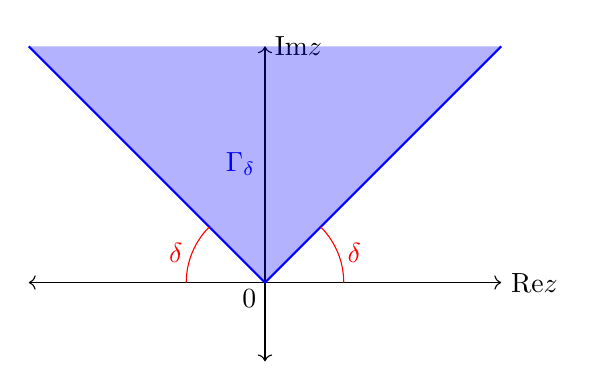
\begin{tikzpicture}[wedge/.style={blue, fill=blue, fill opacity = 0.3},
        angle/.style={red},
        axis/.style={<->,black}]
    %draw axes
    \draw[axis] (-3,0) -- (3,0) node[anchor=west]{$\text{Re} z$};
    \node at (-.2,-.2) {$0$};
    \draw[axis] (0,-1) -- (0,3) node[anchor=west]{$\text{Im} z$};
    %draw wedge
    \fill[wedge] (0, 0) -- (-3, 3) -- (3,3) -- cycle;
    \draw[thick, blue] (-3, 3) -- (0,0) -- (3,3);
    \node[left, blue] at (0,1.5) {$\Gamma_\delta$};
    %draw angle
    \def\ra{.07};
    \draw[red] (1,0) arc (0:45:1) node[midway, right]{$\delta$};
    \draw[red] (-1,0) arc (180:135:1)node[midway, left]{$\delta$};
    \end{tikzpicture}
\end{figure}

When $\mu$ has unbounded support $h_n(z)$ may not be well defined on the real line. We turn to a weaker notion of convergence, namely \textit{non-tangential} limits. For any $0 < \delta < \pi/2$ let $\Gamma_\delta$ be the \textit{wedge} (or \textit{cone}) domain, $\Gamma_\delta = \{\delta < \arg z < \pi - \delta\}$.
Restricting $z$ to $\Gamma_\delta$ gives us the following inequalities for any $x \in \RR$,
\[
    |x - z| \geq |x| \sin \delta 
    \quad\text{and} \quad
    |x - z| \geq |z| \sin \delta.
\]
We will show that
\[
    \lim_{z \rightarrow 0} h_{2n}(z) = 0, \quad z \in \Gamma_\delta
\]
from which the corresponding limit for odd orders will immediately follow from the relation
\[
    h_{2n-1}(z)
    = zh_{2n}(z) + c_{2n}z^{2n}.
\] 
For the sake of convenience we define $w = -\frac1z$. Note that $|w| = \frac1{|z|}$ and if $z$ is in the wedge $\Gamma_\delta$ then so is $w$. Now 
\begin{align*}
    |h_{2n}(z)| 
    &\leq \int_{-\infty}^\infty \frac{|x|^{2n+1}}{|x - w|}d\mu \\
    &\leq \frac{|z|}{\sin \delta} \int_{|x| \leq A} |x|^{2n+1} d\mu
    + \frac1{\sin \delta} \int_{|x| \geq A} x^{2n} d\mu \\
    &\leq \frac{2|z| A^{2n+2}}{\sin \delta}
    + \frac1{\sin \delta} \int_{|x| \geq A} x^{2n} d\mu
\end{align*}
Thus 
\[
    \lim_{z \rightarrow 0} |h_{2n}(z)| \leq \frac1{\sin \delta} \int_{|x| \geq A} x^{2n} d\mu, \quad z \in \Gamma_\delta.
\]
Since $A$ is arbitrary and the integral $\int x^{2n} d\mu = c_{2n}$ is convergent we are done.

Evidently the assymptotic series expansion $g(z) \simeq \sum_{k=0}^\infty c_k (-z)^k$ is generally formal, having zero radius of convergence except in the Markov case. However as we will see in the next section, rational functions constructed from this formal series exist which approximate $g(z)$ on the upper half plane $\{\text{Im} z > 0\}$.

\section{Pad\'e approximants}

In this section we recall the necessary definitions and results. Then we will prove some new results to be applied to the Gaussian Radon transform later.

\begin{definition}[Classical definition of Pad\'e approximants]
The Pad\'e approximant to a (possibly formal) power series 
\[
    R^{[L/M]}(z) \simeq \sum_{k=0}^\infty c_k z^k
\]
is a rational function with nummerator (denominator resp.) degree at most $L$ ($M$ resp.), with series equal to $\sum_{k=0}^N c_k z^k + O(z^{N+1})$ up to as high an order $N$ as possible. 
\end{definition}
Let
\[
    R^{[L/M]}(z) = \frac{P^{[L/M]}(z)}{Q^{[L/M]}(z)} = \frac{a_Lz^L + \cdots + a_1z + a_0}{b_Mz^M + \cdots + b_1z + b_0}.
\]
Notice that in general there is a negligable constant common factor between the numerator and denominator, so that with the remaining $L+M+1$ free parameters, we expect an order of accuracy of up to $L+M+1$ constraints, $c_0, c_1, \ldots, c_{L+M}$. Thus we define the $[L/M]$ Pad\'e approximant by the condition,
\begin{equation}
    \label{eq:BPade}
    \frac{P^{[L/M]}(z)}{Q^{[L/M]}(z)} = \sum_{k=0}^{L+M} c_k z^k + O\left(z^{L+M+1}\right).
\end{equation}
It is helpful to consider the related, and necessary condition
\begin{equation}
    \label{eq:CPade}
    P^{[L/M]}(z) = Q^{[L/M]}(z)\left(\sum_{k=0}^{L+M} c_k z^k\right) + O\left(z^{L+M+1}\right).
\end{equation}
In the classical theory of Pad\'e approximants (\ref{eq:CPade}) was often taken as a definition. It is always possible to find polynomials of the required degree satisfying this second condition, however they do not necessarily attain the degree of accuracy required by the first. We follow Baker, defining $R^{[L/M]}(z)$ by (\ref{eq:BPade}), provided such a rational function exists.

\begin{definition}
    The Pad\'e approximant $R^{[L/M]}$ to a (possibly formal) power series is a the unique rational function with nummerator (denominator resp.) degree at most $L$ ($M$ resp.) satisfying the condition (\ref{eq:BPade}). If no such rational function exists we say the Pad\'e approximant does not exist.
\end{definition}

Here we note that a sufficient condition for the equivalence of the two definitions, and hence for the existence of the Pad\'e approximant by Baker's definition is that $b_0 = Q^{L/M}(0) \neq 0$. 

Equating coeffictients of $z^k$, $k = 0, 1, \ldots, L+M$ in (\ref{eq:CPade}) gives two linear systems
\begin{align*}
    a_0 &= b_0c_0 \\
    a_1 &= b_1c_0 + b_0c_1 \\
    &\vdots \\
    a_L &= b_Lc_0 + b_{L-1}c_1 + \cdots + b_0c_L
\end{align*}
and,
\begin{align*}
    0 &= b_{M}c_{L-M+1} + b_{M-1}c_{L-M+2} + \cdots + b_0c_{L+1} \\
    0 &= b_{M}c_{L-M+2} + b_{M-1}c_{L-M+3} + \cdots + b_0c_{L+2} \\
    &\vdots \\
    0 &= b_{M}c_L + b_{M-1}c_{L+1} + \cdots + b_0c_{L+M}
\end{align*}
where for convenience we set $c_k = 0$ for $k < 0$. The first systems shows the numerator $P^{[L/M]}$ is determined by the denominator $Q^{[L/M]}$. From the second system we can derive a determinantal formula for $Q^{[L/M]}$. Augmented with the desired definition, 
\[
    Q^{[L/M]}(z) = b_Mz^M + b_{M-1}z^{M-1} + \cdots + b_0
\]
the system can be written in the form
\[
    \begin{pmatrix}
        0 \\ 0 \\ \vdots \\ 0 \\ Q^{[L/M]}(z)
    \end{pmatrix}
    =
    \begin{pmatrix}
        c_{L-M+1} & c_{L-M+2} & \cdots & c_{L+1} \\
        c_{L-M+2} & c_{L-M+3} & \cdots & c_{L+2} \\
        \vdots & \vdots & \ddots & \vdots \\
        c_{L} & c_{L+1} & \cdots & c_{L+M} \\
        z^M & z^{M-1} & \cdots & 1
    \end{pmatrix}
    \begin{pmatrix}
        b_M \\ b_{M-1} \\ \vdots \\ b_1 \\ b_0
    \end{pmatrix}
\]
Solving for $b_0$ by Cramer's Rule we get,
% \[
%     b_0 = 
%     \frac{
%         \left|
%         \begin{matrix}
%             c_{L-M+1} & c_{L-M+2} & \cdots & c_L & 0 \\
%             c_{L-M+2} & c_{L-M+3} & \cdots & c_{L+1} & 0 \\
%             \vdots & \vdots & \ddots & \vdots & \vdots \\
%             c_L & c_{L+1} & \cdots & c_{L+M-1} & 0 \\
%             z^M & z^{M-1} & \cdots & z & Q^{[L/M]}(z)
%         \end{matrix}
%         \right|
%     }{
%         \left|
%         \begin{matrix}
%             c_{L-M+1} & c_{L-M+2} & \cdots & c_{L+1} \\
%             c_{L-M+2} & c_{L-M+3} & \cdots & c_{L+2} \\
%             \vdots & \vdots & \ddots & \vdots \\
%             c_{L} & c_{L+1} & \cdots & c_{L+M} \\
%             z^M & z^{M-1} & \cdots & 1
%         \end{matrix}
%         \right|
%     }
% \]

% \[
%     b_0 = 
%     \frac{
%         \left|
%         \begin{matrix}
%             c_{L-M+1} & c_{L-M+2} & \cdots & c_L \\
%             c_{L-M+2} & c_{L-M+3} & \cdots & c_{L+1} \\
%             \vdots & \vdots & \ddots & \vdots  \\
%             c_L & c_{L+1} & \cdots & c_{L+M-1} 
%         \end{matrix}
%         \right| Q^{[L/M]}(z)
%     }{
%         \left|
%         \begin{matrix}
%             c_{L-M+1} & c_{L-M+2} & \cdots & c_{L+1} \\
%             c_{L-M+2} & c_{L-M+3} & \cdots & c_{L+2} \\
%             \vdots & \vdots & \ddots & \vdots \\
%             c_{L} & c_{L+1} & \cdots & c_{L+M} \\
%             z^M & z^{M-1} & \cdots & 1
%         \end{matrix}
%         \right|
%     }
% \]

\[
    b_0
    \left|
    \begin{matrix}
        c_{L-M+1} & c_{L-M+2} & \cdots & c_{L+1} \\
        c_{L-M+2} & c_{L-M+3} & \cdots & c_{L+2} \\
        \vdots & \vdots & \ddots & \vdots \\
        c_{L} & c_{L+1} & \cdots & c_{L+M} \\
        z^M & z^{M-1} & \cdots & 1
    \end{matrix}
    \right|
    =
    \left|
    \begin{matrix}
        c_{L-M+1} & c_{L-M+2} & \cdots & c_L \\
        c_{L-M+2} & c_{L-M+3} & \cdots & c_{L+1} \\
        \vdots & \vdots & \ddots & \vdots  \\
        c_L & c_{L+1} & \cdots & c_{L+M-1} 
    \end{matrix}
    \right| 
    Q^{[L/M]}(z)
\]
The LHS is clearly a polynomial, and nonzero if the RHS minor is nonzero. Thus if the Hankel determinant
\[
    \left|
    \begin{matrix}
        c_{L-M+1} & \cdots & c_L \\
        \vdots & \ddots & \vdots  \\
        c_L & \cdots & c_{L+M-1} 
    \end{matrix}
    \right| 
\]
is nonzero, then up to the afformentioned constant factor,
\begin{equation}
    Q^{[L/M]}(z) = 
    \left|
    \begin{matrix}
        c_{L-M+1} & \cdots & c_{L+1} \\
        \vdots & \ddots & \vdots \\
        c_{L} & \cdots & c_{L+M} \\
        z^M & \cdots & 1
    \end{matrix}
    \right| 
    \label{eq:Qdet}
\end{equation}
By convention we normalize $R^{[L/M]}(z)$ so that $b_0 = Q^{[L/M]}(0) = 1$. 

Since the Hankel determinants give a useful form for expressing some conditions of interest we will difine $H(n,m)$ to be the determinant of the $(m + 1) \times (m + 1)$ Hankel matrix starting with $c_n$,
\[
    H(n,m) :=
    \left|
    \begin{matrix}
        c_{n} & \cdots & c_{n+m} \\
        \vdots & \ddots & \vdots  \\
        c_{n+m} & \cdots & c_{n+2m} 
    \end{matrix}
    \right|
\]
Note in particular that the sufficient condition $Q^{[L/M]}(0) \neq 0$ for the existence of $R^{[L/M]}(z)$ is equivalent to $H(L-M+1, M-1) \neq 0$

We now narrow our focus to Pad\'e approximants to a Humburger series. Let $\mu$ be a positive Borel measure on $\RR$ with infinite support and finite moments $c_k = \int p^k ~d\mu$. Recall that the Hamburger transform of $\mu$,
\[
    g(z) := \int_\RR \frac{d\mu}{1+pz}
\]
has the assymptotic expansion, in the sense of non-tangential limits,
\[
    g(z) \simeq \sum_{k=0}^\infty c_k (-z^k).
\]
We call this formal power series a Hamburger series. 

\begin{remark}
    \tc{To simplify the rest of this maybe we redefine}
    \[
        c_k = (-1)^k\int p^k d\mu
    \]
\end{remark}

\begin{lemma}
    The hamburger moments $c_k$ satisfy the determinental condition $H(2n, m) \neq 0$ for $n,m = 0, 1, \ldots$. 
\end{lemma}
\begin{proof}
    Consider the quadratic form given by
    \[
        G(\mathbf{x}, \mathbf{y}) := 
        \mathbf{x}^\top
        \begin{pmatrix}
            c_{2n} & \cdots & c_{2n+m} \\
            \vdots & \ddots & \vdots  \\
            c_{2n+m} & \cdots & c_{2n+2m}
        \end{pmatrix}
        \mathbf{y}
    \]
    If $\mathbf{x} = (x_0, x_1, \ldots, x_m)^\top$ then
    \begin{align*}
        G(\mathbf{x}, \mathbf{x})
        &= \sum_{i,j=0}^m x_ix_jc_{2n+i+j} \\
        &= \sum_{i,j=0}^m x_ix_j \int p^{2n+i+j} ~d\mu \\
        &= \int \sum_{i,j=0}^m x_ix_jp^{2n+i+j} ~d\mu \\
        &= \int p^{2n}\left(\sum_{k=0}^m x_kp^{k}\right)^2 ~d\mu \geq 0.
    \end{align*}
    Thus $G(\mathbf{x}, \mathbf{y})$ is positive semi-definite. Furthermore, equality holds
    \[
        \int p^{2n}\left(\sum_{k=0}^m x_kp^{k}\right)^2 ~d\mu = 0
    \]
    if and only if $\mu$ is supported entirely on the zeros of the polynomial $p^n\sum_{k=0}^m x_kp^{k}$. However by assumption $\mu$ has infinite support. So in fact $G$ is strictly positive definite. We conclude, by Sylvester's criterion for example, that assocciated hankel matrix has positive determinant. That is, $D(2n, m) > 0$.
\end{proof}

The previous lemma guarentees the existence of certain Pad\'e approximants, specifically those with $L-M+1$ even. 
\begin{theorem}
    If $J$ is odd then the Pad\'e approximant $R^{[L/L+J]}(z)$ to the Hamburger series exists in Baker's sense.
\end{theorem}

% Following Baker's definition [Baker] we say the Pad\'e approximant $R^{[L/M]}$ exists if it satisfies this order of accuracy condition. For details on the construction of Pad\'e approximants see [Baker], []. When the formal series is arbitrary one cannot guarentee the existence of any given $R^{[L/M]}$. However as we will see the situation for Pad\'e approximants to a Hamburger series, for which much is known from the classical theory of moment problems and orthogonal polynomials, is much nicer than the greneral theory.

With our particular application in mind, we will assume the measure $\mu$ is absolutely continuous with respect to the Lebesgue measure and denote it $f(x)dx$ where $f(x)$ is some non-negative Lebesgue measureable function of $\RR$. Let $R_M(z)$ be the "offdiagonal" approximant $R^{[M/M+1]}(z)$ to the Hamburger series of $\mu$,
\[
    R_M(z) = \frac{P_M(z)}{Q_M(z)} \approx \sum_{k=0}^\infty c_k(-z)^k \simeq \int_{-\infty}^\infty \frac{f(p)}{1 + zp} ~dp
\]
where $c_k = \int p^k f(p) dp$. In this section we will prove

\begin{theorem}
    The off-diagonal Pad\'e approximants $R_M(z)$ to the a determinate Hamburger series $\sum_{k=0}^\infty c_k(-z)^k$ exist and converge to $g(z)$ uniformly on compact subsets of the upper half plane $\{\text{Im} ~z > 0\}$.
\end{theorem}

An outline of the proof is as follows: We first justify that the approximants exist in Baker's sense. Then it can be shown that limit of any convergent subsequence of $R_M$ must have a representation as the Hamburger transform of some Borel measure $\mu$ which is a solution to our moment problem, and that furthermore such convergent subsequences exist. Thus in order for the sequence $R_M$ to converge to $g(z)$ it will be necessary and sufficient that the moment problem be determinate.

% Convergence $R_M(z) \rightarrow g(z)$ is \tc{related in some way cant remember} to the determinacy of the moment problem for the sequence $\{c_k\}$. Recall that a moment problem is called determinate if it has a unique solution. \tc{In Akheizer's world, if the moment problem is determinate, then $w_\infty(z)$ is a point for all $z$. Each $R_M$ coresponds to a point $w_M(\omega) = \frac1\omega R_m(-\frac1\omega)$. The points $w_M$ must converge to $w_\infty$}

\begin{proposition}
    If the sequence $c_k$ gives a determinate moment problem then the off-diagonal Pad\'e approximants $R_M(z)$ converge to $g(z)$ locally uniformly.
\end{proposition}

\begin{proof}
    The Pad\'e approximant $R_M(z)$ has a convenient representation as an inner product in terms of a finite Jacobi matrix,
    \[
        R_M(z) = \langle \delta_0, (1 + zA_M)^{-1} \delta_0 \rangle.
    \]
    Now since $A_M$ is a real matrix and $\frac1{|w|} \geq \frac1{|\text{Im}(w)|}$ for any $w \in \CC$, we see that
    \[
        |zR_M(z)| = |\langle \delta_0, (z^{-1} + A_M)^{-1} \delta_0 \rangle| \leq \frac1{|\text{Im}(1/z)|}
    \]
    and thus
    \[
        |R_M(z)| \leq \frac1{|z||\text{Im}(1/z)|} = \frac{|z|}{|\text{Im}(z)|}.
    \]
    Since this bound is independent of $R_M$, Montel's theorem implies that the off-diagonal Pade approximants form a normal family. It can be shown that the limit of any convergent subsequence has a representation $\int (1+ xz)d\sigma(x)$ where $\sigma$ is a solution to the Hamburger moment problem. Since the moment problem is determinate, the sequence $R_M$ must converge to $g(z)$ uniformly on compact sets.
\end{proof}

It remains to discuss the determinacy of the Hamburger moment problem. Here we need to add an additional constraint on the measure $d\mu = f(p)dp$, which is that $f(p)$ is $L^2$ integrable with respect to the Gaussian weight.

\begin{proposition}
    A function $f(p) \in L^2(\mathbb{R}, e^{-p^2}dp)$ such that the moments 
    \begin{equation}
        \label{eq:3}
        c_k = \int_{-\infty}^\infty p^k f(p) e^{-p^2} ~dp, ~ k = 0, 1 \ldots
    \end{equation}
    are finite, is uniquely determined by those moments.
\end{proposition}
    
\begin{proof}
    It is sufficient to show that if $c_k = 0$ for all $k \geq 0$, then $f \equiv 0$ a.e. The Hermite moments are just linear combinations of $0$,
    \[
        \int_{-\infty}^\infty H_k(p) f(p) e^{-p^2} ~dp = 0, ~ k \geq 0
    \]
    where $H_k(p)$ is the Hermite polynomial of order $k$. Since the Hermite polynomials are complete in the space $L^2(\mathbb{R}, e^{-p^2}dp)$ then $f \equiv 0$.
\end{proof}





% % \begin{figure}
% %     \centering
% %     \begin{tikzpicture}
% %         \draw[->] (0, 0) -- (5, 0) node[right] {$x$};
% %         \draw[->] (0, 0) -- (0, 1) node[above] {$y$};
% %         \draw[scale=0.5, domain=1:5, smooth, variable=\x, blue] plot ({\x}, {\x  *exp(-ln(\x))});
% %     \end{tikzpicture}
% % \end{figure}


% Given a formal power series $g(z) = \sum_{k=0}^\infty c_kz^k$ the Pad\'e approximant of degree $[L/M]$ is a rational function whose series expansion agrees with that of $g(z)$ as much as possible, which we denote by $[L/M]_g = \frac{P^{[L/M]}}{Q^{[L/M]}}$ where $P^{[L/M]}(z) = \sum_{k=0}^L a_kz^k$ and $Q^{[L/M]}(z) = \sum_{k=0}^M b_kz^k$ are polynomials of degree at most $L$ and $M$ respectively.  
% \begin{equation}
%     \label{eq:pade}
%     g(z) = [L/M]_g(z) + O(z^{N_{[L/M]}})
% \end{equation}
% Counting unknown coefficients, we can expect an order of accuracy of at most $N_{[L/M]} = L+M+1$. More precisely, we cross multiply and consider the related condition,
% \begin{equation}
%     \label{eq:cross}
%     Q^{[L/M]}(z)g(z) - P^{[L/M]}(z) = O(z^{L+M+1}),
% \end{equation}
% which can be written as a system of $L + M + 1$ linear equations
% \begin{align*}
%     \sum_{\ell = 0}^k b_\ell c_{k-\ell} &= a_k & k &= 0, 1, \ldots, L \\
%     \sum_{\ell = 0}^k b_\ell c_{k-\ell} &= 0, & k &= L + 1 \ldots, L + M
% \end{align*}
% where for convenience we set $b_\ell = 0$, $\ell > M$ and $c_\ell = 0$, $\ell < 0$. Thus a solution $b_0, \ldots, b_M$ can be found to a underdetermined homogeneous system of $M$ equations in $M+1$ unknowns, and then $a_0, \ldots, a_L$ can be computed directly. The rational function $\frac{P^{[L/M]}}{Q^{[L/M]}}$ has an irreducible form $\frac{P_\star^{[L/M]}}{Q_\star^{[L/M]}}$ which can be normalized so that $Q_\star^{[L/M]}(0) = 1$. Subject to these constraints this defines a unique rational approximation satisfying (\ref{eq:cross}) and from now the notation $[L/M]_g$ will refer to the unique normalized irreducible form $\frac{P_\star^{[L/M]}}{Q_\star^{[L/M]}}$. Note that $[L/M]_g$ computed in this way may not satisfy (\ref{eq:pade}) up to the desired order $L+M+1$, particularly in the case when $Q^{[L/M]}(0)=0$. In the event that no rational function of degree $[L/M]$ exists approximating $g$ to the desired accuracy we say the $[L/M]$ Pad\'e approximant does not exist. We will focus on cases where they do exist. Besides, in general it can be shown that infinitely many approximants exist in a sense in which we can move on to talking about convergence.

% The convergence of Pad\'e approximants is  not fully understood in general. We will concern ourselves with a particular case for which these questions have answers: approximants on a diagonal, $[m+k/m]$ as $m \rightarrow \infty$ for certain integral forms.


% Now consider the function defined by
% \[
%     g(z) = \int_{-\infty}^\infty \frac{GR_f(\omega, p)e^{-p^2}}{1 - zp} ~dp
% \]
% which has an at least formal expansion
% \[
%     g(z) \simeq \sum_{n=0}^\infty c_kz^k
% \]
% where
% \[
%     c_k = \int_{-\infty}^\infty p^k GR_f(\omega, p)e^{-p^2} ~dp.
% \]

% In this case question of the convergence $[L/M]_g \rightarrow g$ is related to whether this Hamburger moment problem is determinate.
% \begin{proposition}
% A function $f(p) \in L^2(\mathbb{R}, e^{-p^2}dp)$ such that the moments 
% \begin{equation}
%     \label{eq:3}
%     c_k = \int_{-\infty}^\infty p^k f(p) e^{-p^2} ~dp, ~ k = 0, 1 \ldots
% \end{equation}
% are finite, is uniquely determined by those moments.
% \end{proposition}

% \begin{proof}
%     It is sufficient to show that if $c_k = 0$ for all $k \geq 0$, then $f \equiv 0$ a.e. The Hermite moments are just linear combinations of $0$,
% \[
%     \int_{-\infty}^\infty H_k(p) f(p) e^{-p^2} ~dp = 0, ~ k \geq 0
% \]
% where $H_k(p)$ is the Hermite polynomial of order $k$. Since the Hermite polynomials are complete in the space $L^2(\mathbb{R}, e^{-p^2}dp)$ then $f \equiv 0$.
% \end{proof}

% \tc{My understanding here is that since the moments $c_k$ uniquely determine $GR_f(\omega, p)$, and thus $g(z)$, then the Pad\'e approximants, if they converge, must converge to $g(z)$. Correct?}


% We will now (attempt to) define a multivariate analogue to the Pad\'e approximants. We'll detail the bivariate case for example and promise that higher dimensions follow similarly. Informally, a multivariate power series is written as a sum of homogeneous polynomials, the Pad\'e approximants similarly decomposed into homogeneous polynomials. A system of linear equations is formed nearly identical to that of the classical Pad\'e approximants, but with somewhat more unknowns. A "degree shift" by $LM$ is necessary to ensure the system has a nontrivial solution. According to Cuyt the structure of this system (so called "near Toeplitz") reduces the complexity for computing solutions from $O(n^3)$ to $O(\alpha n^2)$ where $n$ is the dimension of the system and $\alpha$ is its "displacement rank." As in the univariate case it is shown these Pad\'e approximants have a unique reduced form up to a normalization constant.

% \tc{I obviously need to fill in a lot more detail here. The "degree shift" is currently what is confusing me...}

% Let me be more specific... \tc{use multi-index notation? Probably not necessary, but it looks cleaner.} Consider a formal power series in the variable $x = (x_1, \ldots, x_d) \in \mathbb{R}^d$
% \[
%     g(x) = \sum_{\alpha_1, \ldots, \alpha_d = 0}^\infty c_{\alpha_1, \ldots, \alpha_d} x_1^{\alpha_1}\cdots x_d^{\alpha_d} = \sum_{\ell = 0}^\infty C_\ell(x)
% \]
% where $C_\ell(x^\ell)$ is a homogeneous polynomial in the coordinates of $x$,
% \[
%     C_\ell(x) := \sum_{\alpha_1 + \cdots + \alpha_d = \ell} c_{\alpha_1, \ldots, \alpha_d} x_1^{\alpha_1}\cdots x_d^{\alpha_d}.
% \]
% Similarly to the univariate case we seek a rational function $[L/M]_g = \frac{P^{[L/M]}}{Q^{[L/M]}}$ where
% \[
%     P^{[L/M]}(x) 
%     % = \sum_{|\alpha| \leq L} a_\alpha x^\alpha
%     = \sum_{\ell = LM}^{LM + L} A_\ell(x)
%     = \sum_{\ell = LM}^{LM + L} \sum_{|\alpha| = \ell} a_\alpha x^\alpha
% \]
% \[
%     Q^{[L/M]}(x) 
%     % = \sum_{|\alpha| \leq M} b_\alpha x^\alpha
%     = \sum_{\ell = LM}^{LM + M} B_\ell(x)
%     = \sum_{\ell = LM}^{LM + M} \sum_{|\alpha| = \ell} b_\alpha x^\alpha
% \]
% such that
% \[
%     g(x) = [L/M]_g(x) + O(x^\alpha, |\alpha| \geq LM + L + M + 1).
% \]
% Note the "degree shift" by $LM$, which is necessary to guarantee nontrivial solutions. Following the univariate case we cross multiply and consider the accuracy through order condition
% \begin{equation}
%     \label{eq:multicross}
%     Q^{[L/M]}(x)g(x) - P^{[L/M]}(x) = O(z^{LM + L+M+1}),
% \end{equation}
% which once again gives $Q^{[L/M]}(x)$ as a solution to an underdetermined (because of the degree shift) homogeneous system of linear equations, and $P^{L/M}(x)$ is computed from the remaining equations. 

% A useful note about the homogeneous form for the power series, which we will use later, is that when restricted to the slice $x = p\omega$ for a fixed unit vector $\omega \in \mathbb{R}^n$ it is easily expressed as a power series in $p$,
% \[
%     \sum_{\ell = 0}^\infty C_\ell(p\omega)
%     = \sum_{\ell = 0}^\infty C_\ell(\omega) p^\ell
% \]
% and similarly for the polynomials.
% \tc{[Note to self and Maxim] This seems to be the crux of the "powerful slice theorem" for homogeneous Pad\'e approximant (Cuyt's Theorem 2). The degree shift, which just adjusts the dimensions of the linear system to guarantee a nontrivial solution, reduces on slices: if $P^{[L/M]}(x) = \sum_{\ell = LM}^{LM+L}A_\ell(x)$, $Q^{[L/M]}(x) = \sum_{\ell = LM}^{LM+M} B_\ell(x)$ then
% \[
%     \frac{P^{[L/M]}(p\omega)}{Q^{[L/M]}(p\omega)}
%     = \frac{\sum_{\ell = LM}^{LM+L}A_\ell(\omega)p^{\ell}}{\sum_{\ell = LM}^{LM+M}B_\ell(\omega)p^{\ell}}
%     = \frac{\sum_{\ell = 0}^{L}A_{LM+\ell}(\omega)p^\ell}{\sum_{\ell = 0}^{M}B_{LM+\ell}(\omega)p^\ell}
% \]
% the RHS satisfies the "accuracy through order condition" (\ref{eq:cross})... 
% \begin{align*}
%     \left(\sum_{\ell=0}^\infty C_{\ell}(\omega)p^\ell\right)
%     \left(\sum_{\ell=0}^M B_{LM+\ell}(\omega)p^\ell\right) -
%     \sum_{\ell=0}^L A_{LM+\ell}(\omega)p^\ell \\
%     = \frac1{p^{LM}} \left(g(p\omega) Q^{[L/M]}(p\omega) - P^{[L/M]}(p\omega)\right)
%     = O(p^{L+M+1})
% \end{align*}
% and thus in irreducible form is equal to the unique univariate Pad\'e approximant for $g_\omega(p) := g(p\omega)$. On a personal note it is so much clearer to write this out with the general degree $[L/M]$ as opposed to $[m + k/m]$. The proof above would work for any degree shift, so long as the multivariate pade order through accuracy condition is satisfied.}

% \tc{...insert the construction of multi pade}

\section{Convergence results for the Gaussian Radon transform}
% What is the relationship between the Gaussian and Classical Radon Transform
% \[
%     GR_f(\omega, p)e^{-p^2/2} 
%     = e^{-p^2/2} \int_{\langle x, \omega \rangle = p} e^{-|p\omega-x|^2/2} f(x) dx
%     = \int_{\langle x, \omega \rangle = p} e^{-|x|^2/2} f(x) dx
%     = R_g(\omega, p)
% \]
% where $g(x) = e^{-|x|^2/2} f(x)$

% \begin{tikzcd}
%     f \arrow[d, "\psi"] \arrow[r, "\eta"]
%     & Gf \arrow[d, "\psi"] \\
%     R_f \arrow[r, "\eta"]
%     & GR_f
% \end{tikzcd}



Now we are in the position to assemble all the previous results into an approximation scheme to be used for reconstruction shapes of unbounded domains.

Take a non-negative Lebesgue measureable function $f(x)$ on $\RR^n$ with finite multivariate Gaussian moments
\[
    c^G_\alpha = \int_{\RR^n} f(x)e^{-\|x\|/2} x^\alpha dx
\]
We have seen that the multivariate Stieltjes transform of $f$, 
\[
    g(z) = \int_{\RR^n} \frac{f(x)e^{-\|x\|/2}}{1 + \langle x, \omega \rangle z} dx,
\]
is equal to the Hamburger transform of $GR_f(\omega, p)$, whose moments in turn are easily computed from the moments of $f$, for fixed $\omega$. Thus for $z$ in the one dimensional subspace spanned by $\omega$, $g(z)$ can be approximated well by Pad\'e approximants, under the integrability condition $GR_f(\omega, p) \in L^2(\RR, e^{-p^2}~dp)$. On the other hand as an integral on $\RR^n$, we can also approximate $g(z)$ by cubature formula,
\[
    \int_{\RR^n} \frac{f(x)e^{-\|x\|^2/2}}{1 + \langle x, \omega \rangle z} dx 
    \approx \sum_{\ell = L} \frac{e^{-\|x_\ell\|^2/2}}{1 + \langle x_\ell, \omega \rangle z} w_\ell f(x_\ell)
    =: \sum_{\ell = L} C_\ell(z) f(x_\ell).
\]
By equating these parallel approximations, 
\[
    \sum_{\ell = L} C_\ell(z) f(x_\ell) \approx R_M(z),
\]
with a sufficient quantity of sample points $z_j$ we have arrived at a linear system
\[
    \sum_{\ell = L} C_\ell(z_j) f(x_\ell) = R_M(z_j), 
    \qquad j = 1, 2, \ldots, J
\]
from which we should be able to recover the value of $f$ on our cubature nodes $x_\ell$.



% We have seen that the Hamburger transform of the GRT of $f$,
% \[
%     g(z) = \int_{-\infty}^\infty \frac{GR_f(\omega, p) e^{-p^2/2}}{1 + pz}dp
% \]
% can be approximated to an arbitrary degree by offdiagonal Pad\'e approximants, $R_M(z)$ near zero. On the other hand as an integral over $p$


\section{An example}

For a simple example let $n = 2$ and let $f(x)$ be the charactaristic function of an infinite "strip" of unit width centered on the origin and perpendicular to $\varphi \in S^1$:
\[
    f(x) =
    \begin{cases}
        1, & \langle x, \varphi \rangle \leq 1/2 \\
        0, & \text{otherwise}
    \end{cases}
\]

Unit ball in $\RR^3$? Annulus in $\RR^2$? Some assymmetric or off-center examples?


% \section{Radon transform picture}

 
%  %\begin{wrapfigure}{l}{0.2\textwidth}
%   %\begin{center}
% \resizebox{.5 \textwidth}{!}{%

%      \begin{tikzpicture}[scale=2, rotate=-30]  
   

% \coordinate (A) at (0,0);

% \coordinate (B) at (0,1.5);

% \coordinate (C) at (1,0);

% \coordinate (D) at (0.5,0.5);

% \coordinate (E) at (0.5,2);

% \coordinate (F) at (1.5,0.5);

% \coordinate (G) at (-1,0);

% \coordinate (H) at (-0.5,0.5); 

% \coordinate (I) at (0,-0.25); 
% \coordinate (J) at (0.5,0.25); 

 




 

% \shadedraw[blue, rotate=30] (G)--(A)--(C)--(F)--(D)--(H)--(G);

% \draw[blue] (-.75,.15)--(.5,.45);
% \draw[blue] (.5,.15)--(.75,.45);
%  \coordinate [label=left:\textcolor{purple}{${}_L$}] (P) at (0.5,0.25);
 
 

 
%  \coordinate [label=below:\textcolor{purple}{$ {Rf(L)= \int_Lf(x)\,dx}$}] (u) at (.5,0.15);
 

% %\draw[blue] (A)--(D);
 
% %\draw[->](O)--(u);

 

%  \end{tikzpicture}
%  }
 %\end{center}
 %\end{wrapfigure}
 


\end{document}
